\documentclass[10pt]{article}

\usepackage[margin=0.7in]{geometry}
\usepackage{graphicx}
\usepackage{hyperref}

\begin{document}

\hfill Sigitas Rimkus \qquad Daniel Geiyer
\section*{Progress Report 2}
\subsection*{Reiteration of project idea and goals}
We propose to analyze the vibrational properties of a rectangular membrane.  Specifically, we are interested in finding the first several mode shapes of this membrane using an FEA software package and validating those results using analytical solutions.  After receiving feedback from the first progress report, we realized that an increase in problem difficulty is required.  Therefore, we propose adding the following to our project goals:
\begin{itemize}
	\item{Perform the same vibration analysis as above, but with various boundary conditions (i.e. one edge free, two edges free, etc.)}
	\item{Perform the same vibration analysis as above, but with holes of various geometries and sizes cut out of the membrane.}
\end{itemize}

\subsection*{FEA Modeling Method}
The following itemizes the details and general procedures of how we plan on implementing our FEA solution.
\begin{itemize}
	\item{The model will be a 2D plane}
	\item{At first, we will use quadrilateral, 8-node elements}
	\begin{itemize}
		\item{Other nodes we may choose to include for solution accuracy include 4-node quadrilaterals, shells, and triangles}
	\end{itemize}
	\item{Initial model will have no thickness, but future iterations may have thickness much less than the widths of the membrane.}
	\item{Model will be square with arbitrary dimensions (irrelevant for mode shapes) with all sides fixed.}
	\item{Material properties are currently unspecified, but we would like to relate model to a practical application through the choice of material, for example modeling the behavior of a drumhead.}
	\item{Fine meshed will be applied with no additional loading conditions.}
	\item{Some FEA software packages allow for animations of mode shapes.  We will include these for the presentation if NASTRAN has this capability.}
	\item{Complexity will be added to future model iterations to simulate real-world problems.}
\end{itemize}
\begin{figure}[h]
	\centering
	\includegraphics[width=0.4\textwidth]{Constrained7}
	\caption{Example meshing of a square membrane in ANSYS (source: \url{http://www.mece.ualberta.ca/tutorials/ansys/AT/BirthDeath/images/Constrained7.gif}}
\end{figure}

\subsection*{Validation of FEA results}
The bulk of the work for analytically validating the FEA results for mode shapes has been completed.  The wave equation was used and subsequently solved for the case when all four edges of the membrane are clamped.
\begin{figure}[h]
	\centering
	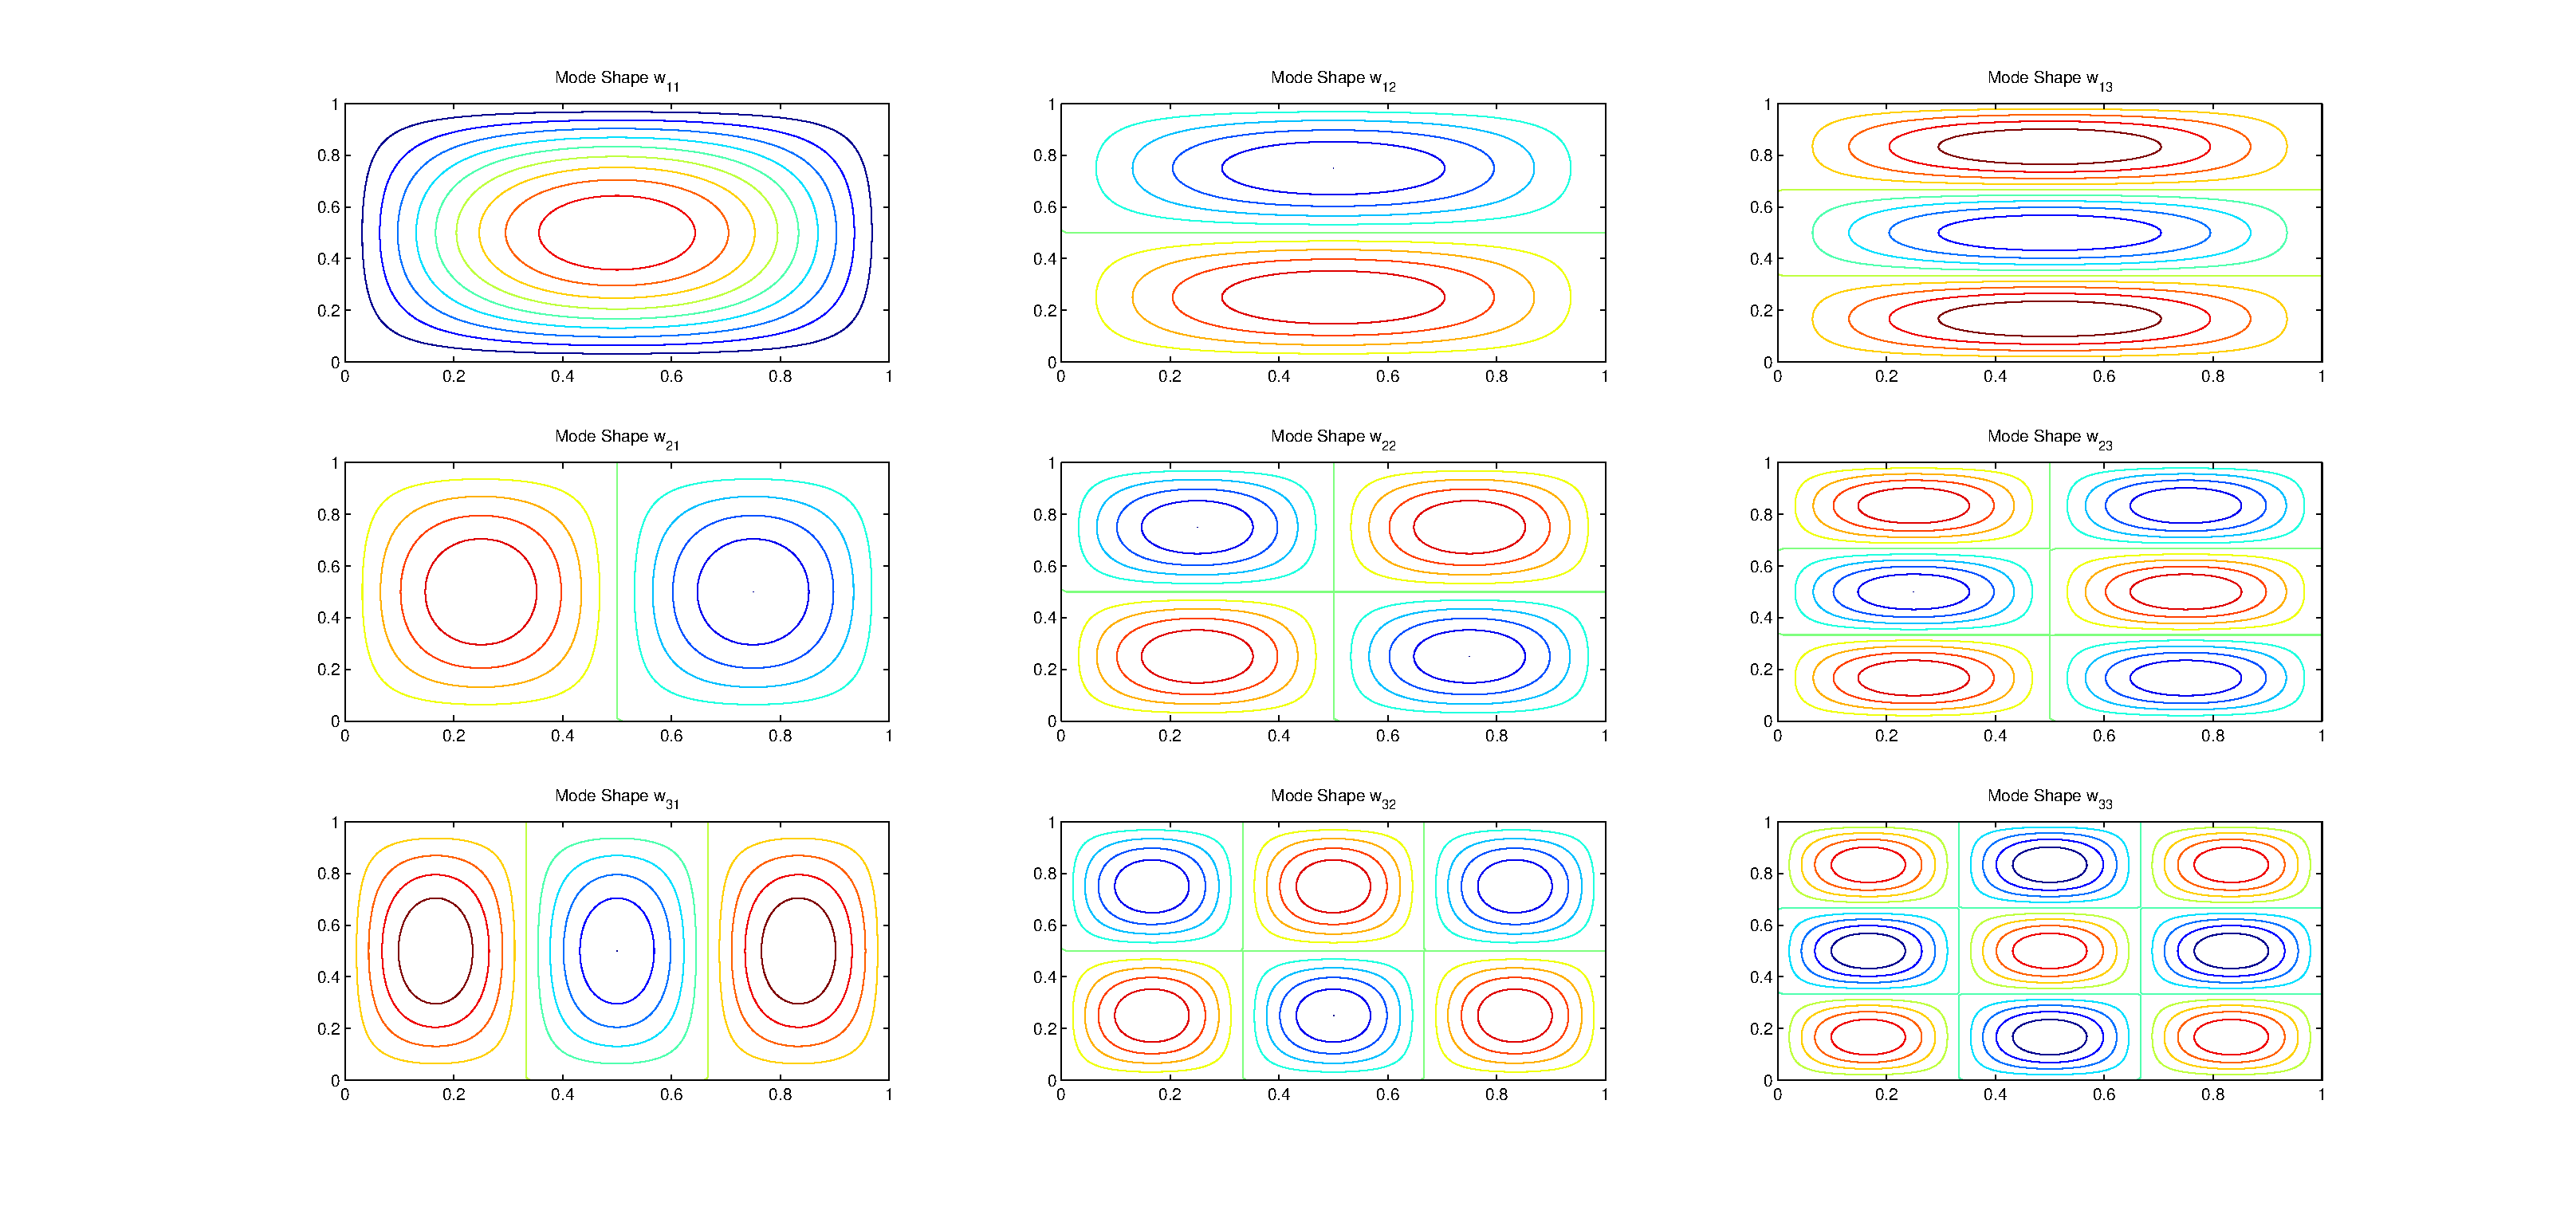
\includegraphics[width=\textwidth]{modes}
	\caption{The selected mode shapes used to validate the FEA results (contours generated with MATLAB)}
\end{figure}
In addition to the majority of the analytical work being completed, a MATLAB script has been written to generate contour plots (such as the one above) as well as surface plots of the selected mode shapes.  We have yet to decide how we plan on validating the cases where the membrane model is more complex (such as various boundary conditions, or when there are holes in the membrane).

\subsection*{Next steps}
Aside from obtaining FEA results, which shouldn't be too difficult, we have several items left to complete.  First, we need to finish writing the report.  Once the FEA results have been obtained, they can be quickly incorporated into this document.  Second, we need to finish our presentation slides.  This too will be complete once the FEA results are in.

\end{document}
